% !TeX root = ./pf2022.tex

%\includeonlyframes{current}

\section{Basics}

\begin{frame}{The language of a computer}
  \begin{itemize}[<+->]
  \item A \textit{computer} is a device that executes programs
  \item A \textit{program} is a collection of instructions to perform a specific
    task
  \item For a computer to understand instructions, these need to be expressed in a
    language that the computer can understand
  \end{itemize}

\end{frame}

\begin{frame}[fragile]{Binary language}

\begin{semiverbatim}
{\color{gray}\tikzref{markbit}0010\tikzref{markbyte}1001110110011000011111010111001011100111101100
11101000101001101011100111111100011101001000011010
00000110001101000011111010010001000101110000010010
00111011010111101101111110110011011111101100101101
10010010110011001101110011000011001011000001010010
11110100101111010001111001011000000000001111110100
1001110101100011010100\tikzref{ins}011100000001\tikzref{ins2}11000011\tikzref{ins3}01001101
00010001111001101000111100100110110110001101100100
01000110010111100011100010100101011011000110010001
10100011111101101000000000111101000001000100101101
11101100011010111001111110010101010110010010000100
00000010010011111010111011011101110011101100000111
00001001111011000000110000100110000101000100111011}\end{semiverbatim}

\uncover<2->{
  \uncover<2->{\tikz[overlay] \node[draw,rounded corners,thick,green,minimum
  width=3mm,minimum height=5mm,label={\color{green}bit}] (bit) at ([xshift=.5ex]markbit) {};}
  \uncover<3->{\tikz[overlay] \node[draw,rounded corners,thick,blue,minimum
  width=17mm,minimum height=7mm,label={45:{\color{blue}byte (8 bits)}}] (byte) at ([xshift=-.4ex]markbyte) {};}
  \uncover<4->{\tikz[overlay] \node[draw,rounded corners,thick,red,minimum width=49mm,minimum height=5mm] (instruction) at (ins) {};
  \tikz[overlay] \node[red] (description) at ([yshift=-32mm]instruction.south) {increment a number by 1 (for an x86_64)};
  \tikz[overlay] \draw[<-,red,thick] (instruction) -- (description);}
}

\end{frame}

\begin{frame}[fragile]{Programming language}
  \begin{itemize}
  \item<1-> A (high-level) programming language is an artificial language to write
    programs that is closer to humans
    \begin{columns}
      \begin{column}{.5\textwidth}
    \begin{codeblock}
int increment(int n)
\{
  return n + 1;
\}\end{codeblock}        
      \end{column}
      \begin{column}{.5\textwidth}
        {\smaller More or less equivalent to the function}
        \[
          \verb|increment|(n) = n + 1 \quad \forall n \in \mathbb{Z}
        \]
      \end{column}
    \end{columns}
\item<2-> Some form of translation needs to be applied to the program written in a
  high-level language to transform it into a program expressed in a binary
  language
\item<3-> To complicate things, the binary language is architecture-specific
  \begin{itemize}[<.->]
  \item Many architectures (Instruction Set Architectures -- ISA) have been
    defined over the years, many still in use
  \item i386, \textbf{x86_64}, SPARC, MIPS, \textbf{ARM}, VAX, Alpha, RiscV,
    PowerPC, \ldots
  \end{itemize}
\item<4-> The translation is done by other programs, for example
  \alert{compilers} and interpreters
\end{itemize}

\end{frame}

\begin{frame}{C++}

  \begin{itemize}[<+->]
  \item There are many programming languages, with very different characteristics
  \item Why \Cpp{}?
    \begin{itemize}[<.->]
    \item general purpose
    \item support for multiple styles of programming (\textit{paradigms})
    \item much used in scientific fields, but also in games, finance,
      telecommunications, embedded, \ldots
    \item available on all platforms
    \item efficient
    \item ISO standard
    \end{itemize}
  \end{itemize}
\end{frame}

\begin{frame}{Many types of computers}

  \begin{columns}

    \begin{column}{.5\textwidth}

      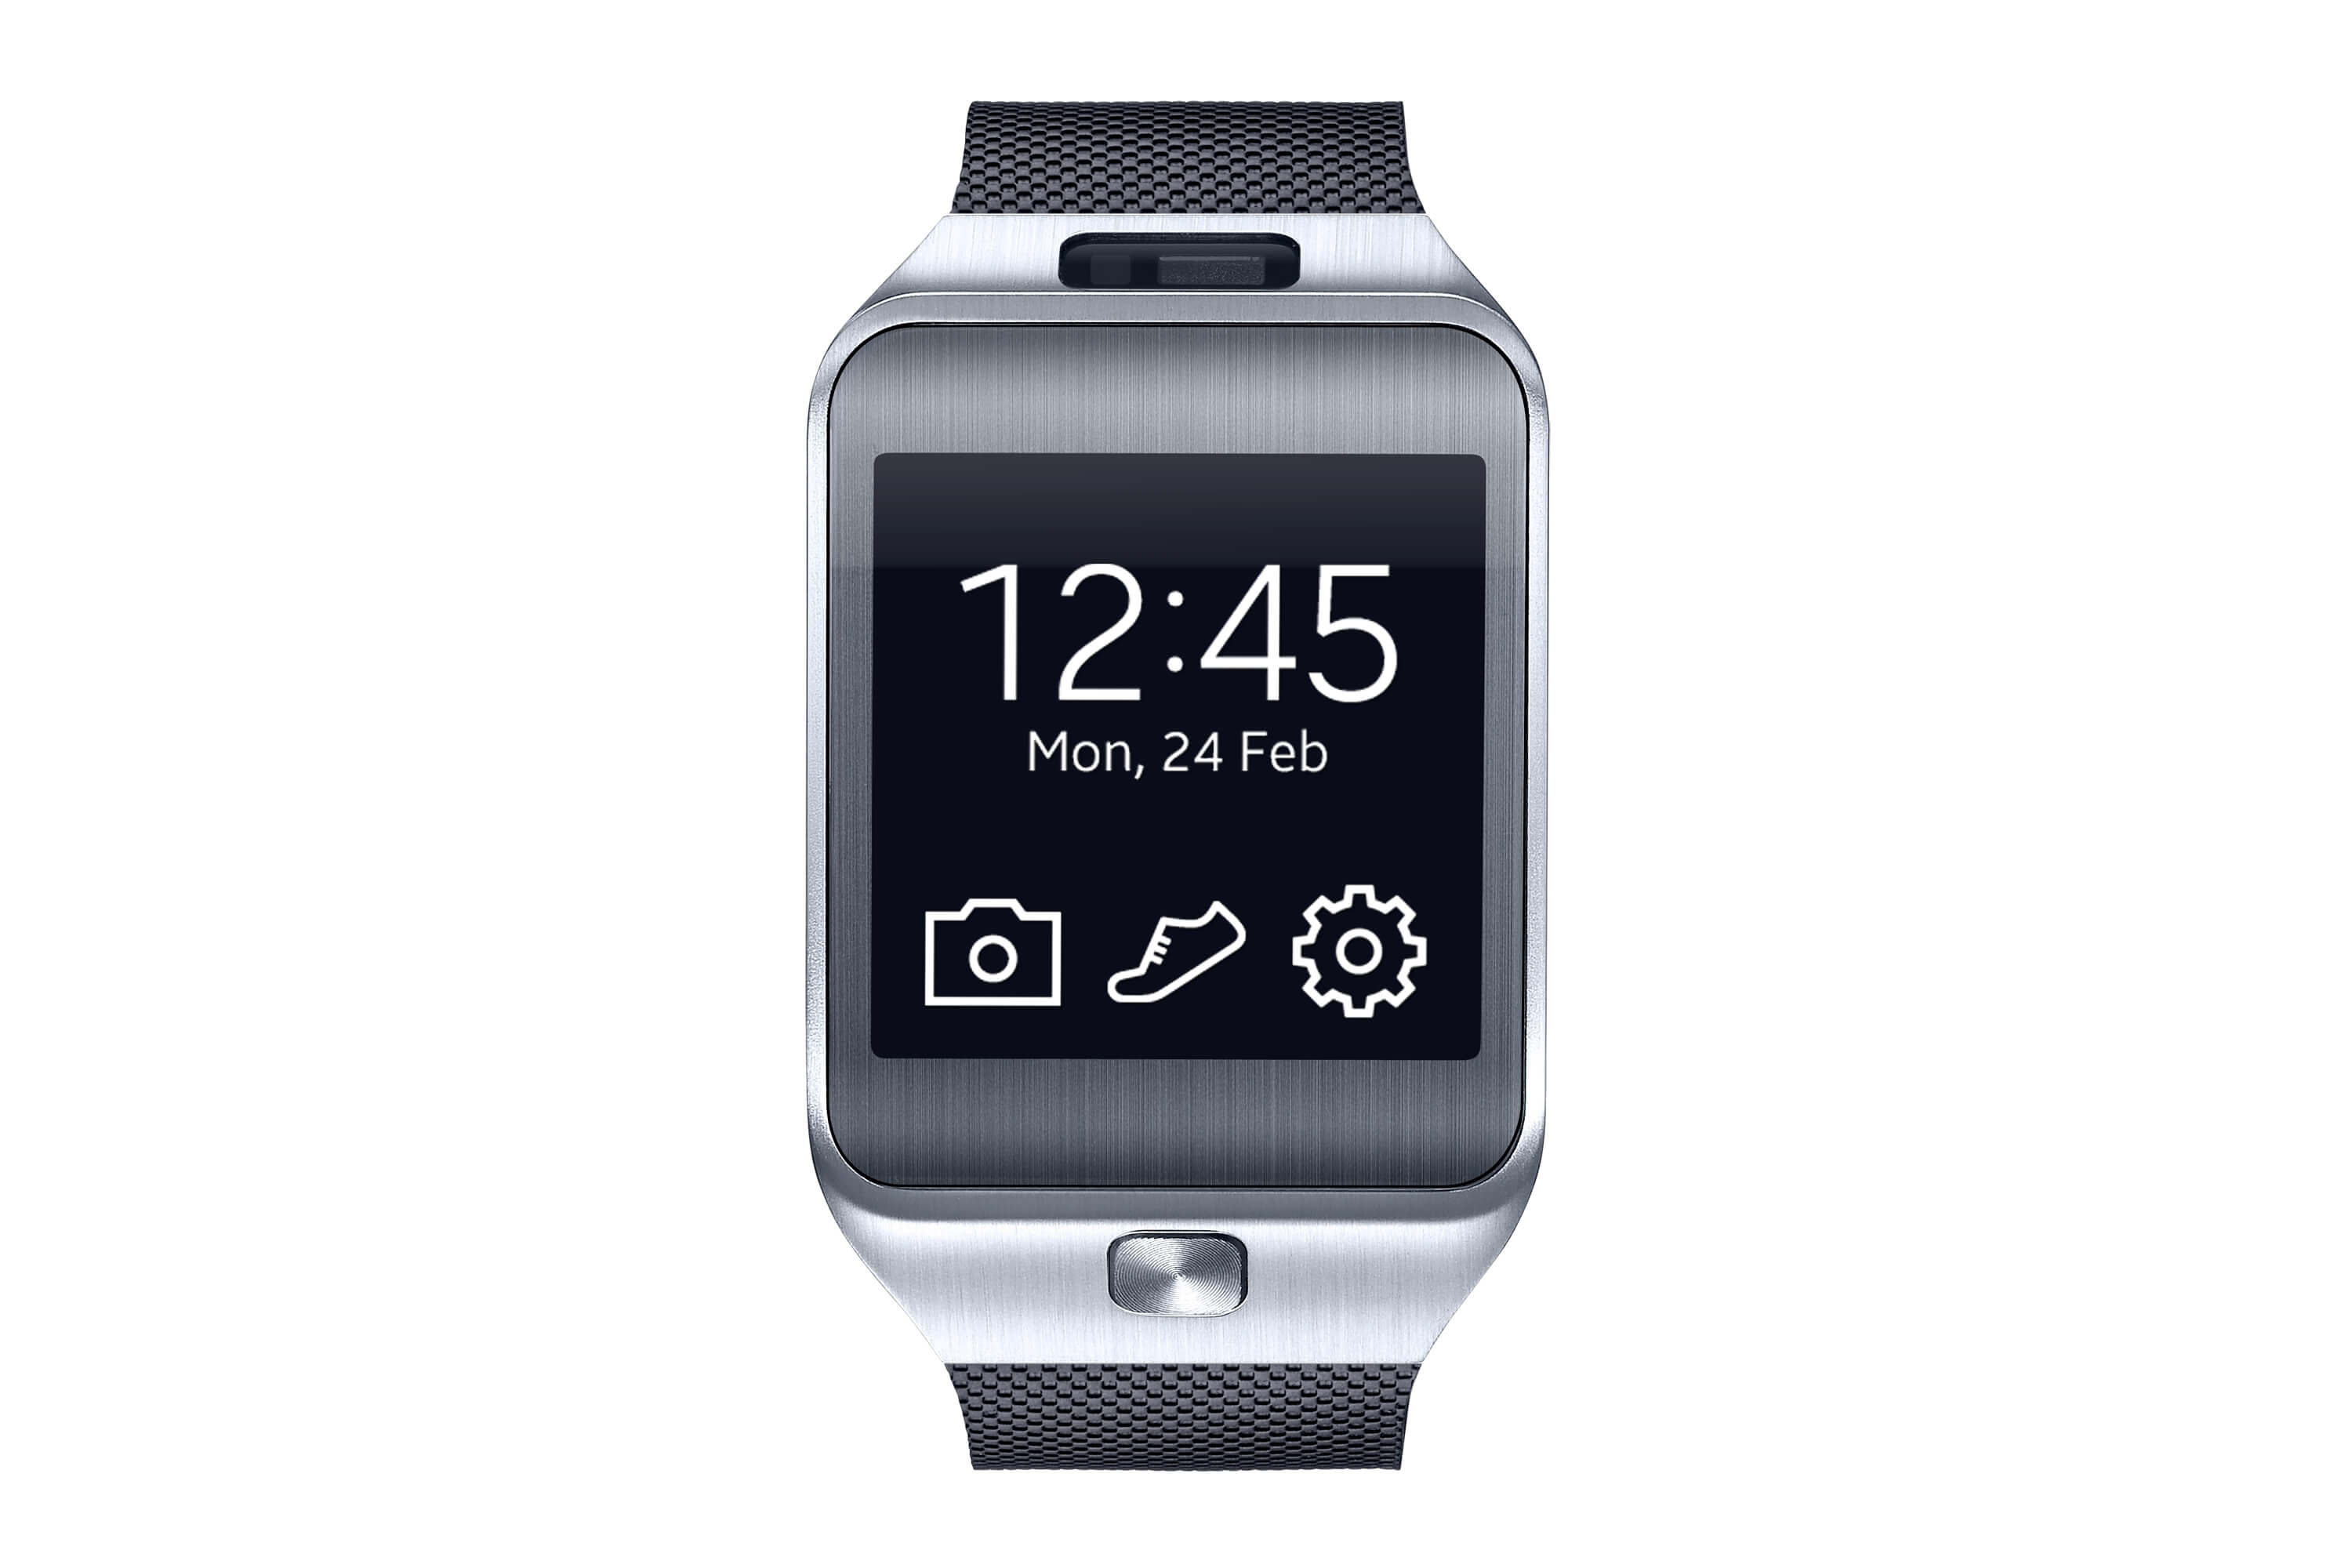
\includegraphics[width=\textwidth]{images/samsung-gear-compressed.jpeg}

      \begin{center}
        {\tiny(from \url{https://www.samsung.com/})}
      \end{center}
    \end{column}

    \begin{column}{.5\textwidth}
      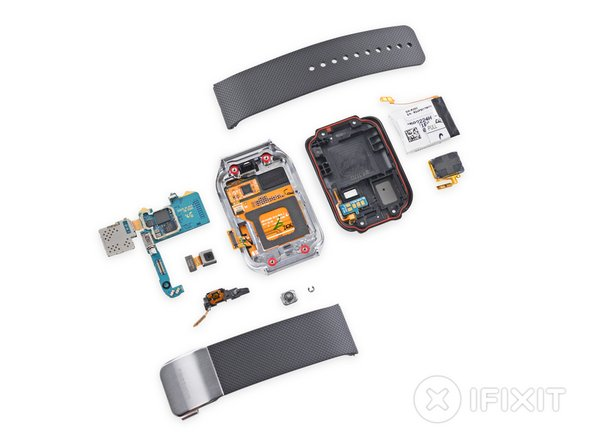
\includegraphics[width=\textwidth]{images/gear2-ifixit.jpg}

      \begin{center}
        {\tiny (from \url{https://www.ifixit.com/})}
      \end{center}
    \end{column}

  \end{columns}

\end{frame}

\begin{frame}{Many types of computers \insertcontinuationtext}
  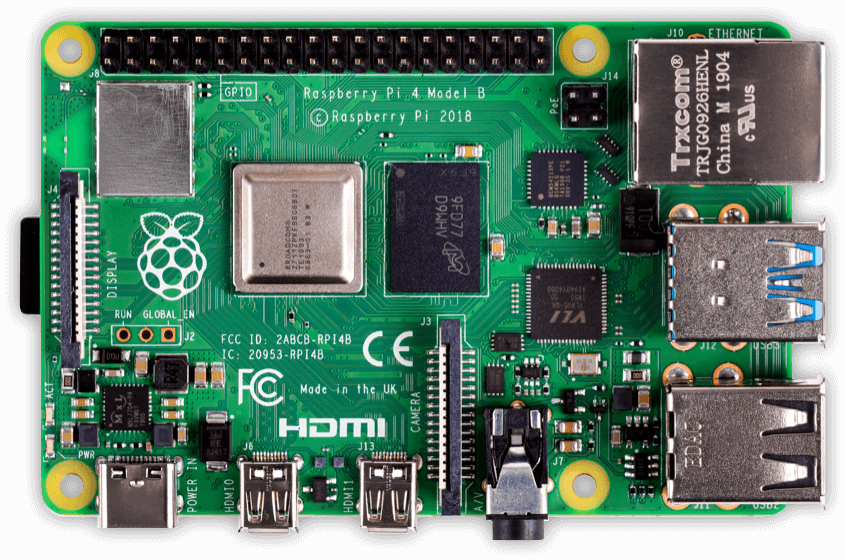
\includegraphics[width=\textwidth]{images/rpi-compressed.png}

  {\tiny (from \url{https://www.raspberrypi.org/})}
\end{frame}

\begin{frame}{Many types of computers \insertcontinuationtext}
  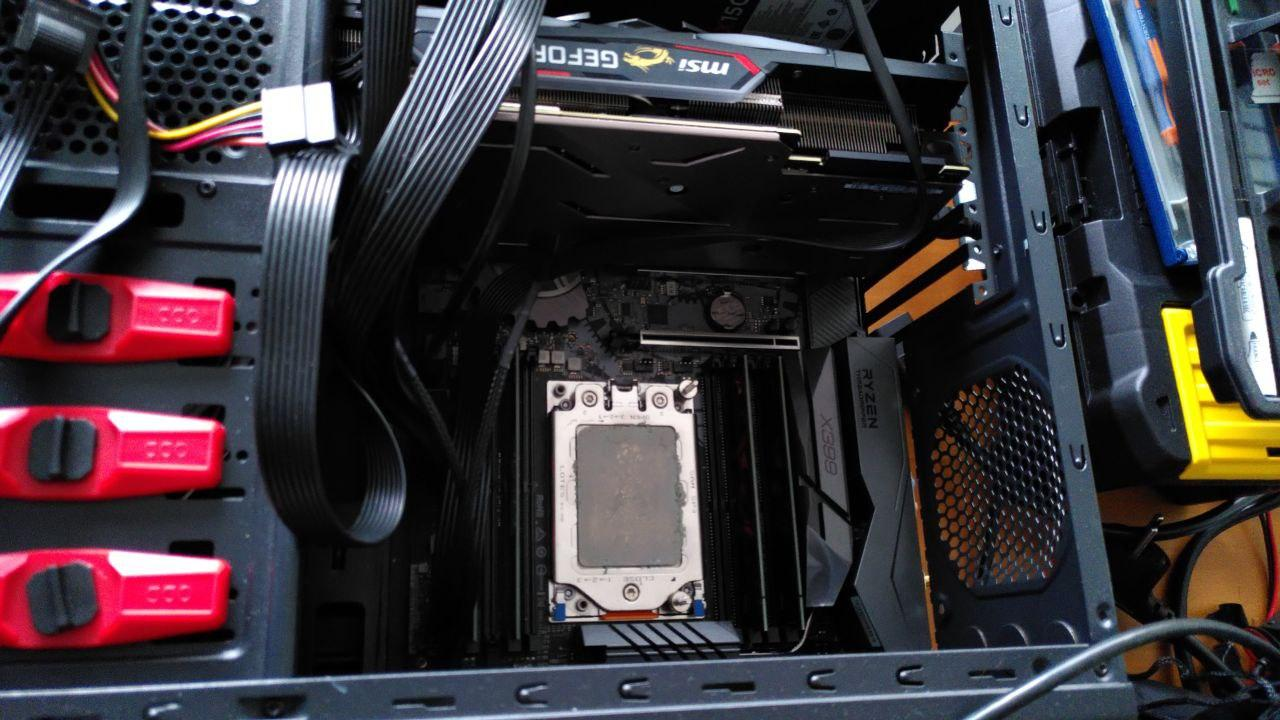
\includegraphics[width=\textwidth]{images/desktop.jpg}
\end{frame}

\begin{frame}{Many types of computers \insertcontinuationtext}
  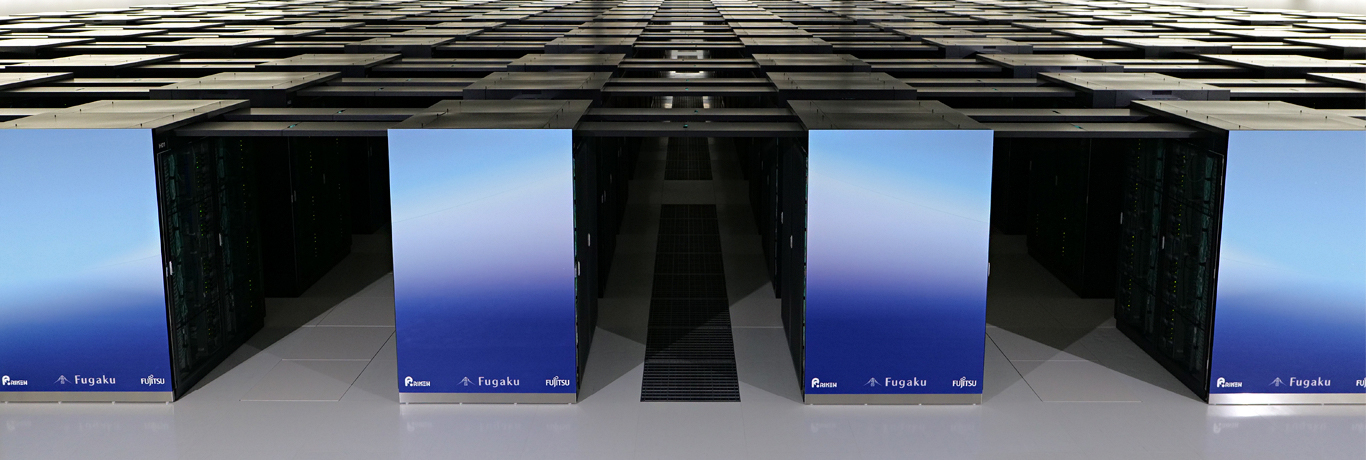
\includegraphics[width=\textwidth]{images/fugaku.jpg}

  {\tiny (from \url{https://www.riken.jp/en/})}
\end{frame}

\begin{frame}{The Von Neumann architecture}

  \begin{center}

    \vskip -.8cm

    \begin{tikzpicture}[every text node part/.style={align=center}]
      \uncover<3->{
        \node[rectangle,draw,thick,minimum height=4cm,minimum width=2.1cm,fill=yellow,"Memory"] (memory) {
          data \\ + \\ instructions
        };
        \node[above=20pt of memory,inner sep=0pt,outer sep=0pt] (ram) {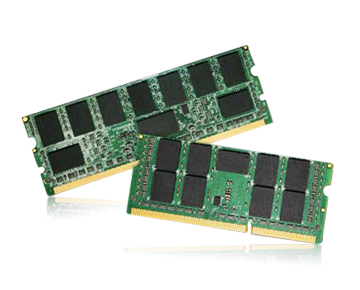
\includegraphics[height=1cm]{images/ram.jpg}};
      }
      \uncover<2->{
        \node[rectangle,black,draw,thick,minimum height=4cm,minimum width=2.5cm,fill=red!80!black,right=of memory,"CPU"] (cpu) {};
        \node[rectangle,black,draw,thick,text width=2cm,minimum
        height=1cm,fill=white,below=10pt of cpu.north,inner sep=0pt,outer sep=0pt] (alu) {\scriptsize
          Arithmetic-Logic Unit};
        \node[rectangle,black,draw,thick,minimum width=2cm,fill=white,above=of cpu.south] (control) {\scriptsize Control};
        \path (alu) -- (control) node[midway,rectangle,black,draw,thick,minimum width=2cm,fill=white] (registers) {\scriptsize Registers};
        \node[above=20pt of cpu,inner sep=0pt,outer sep=0pt] (intel) {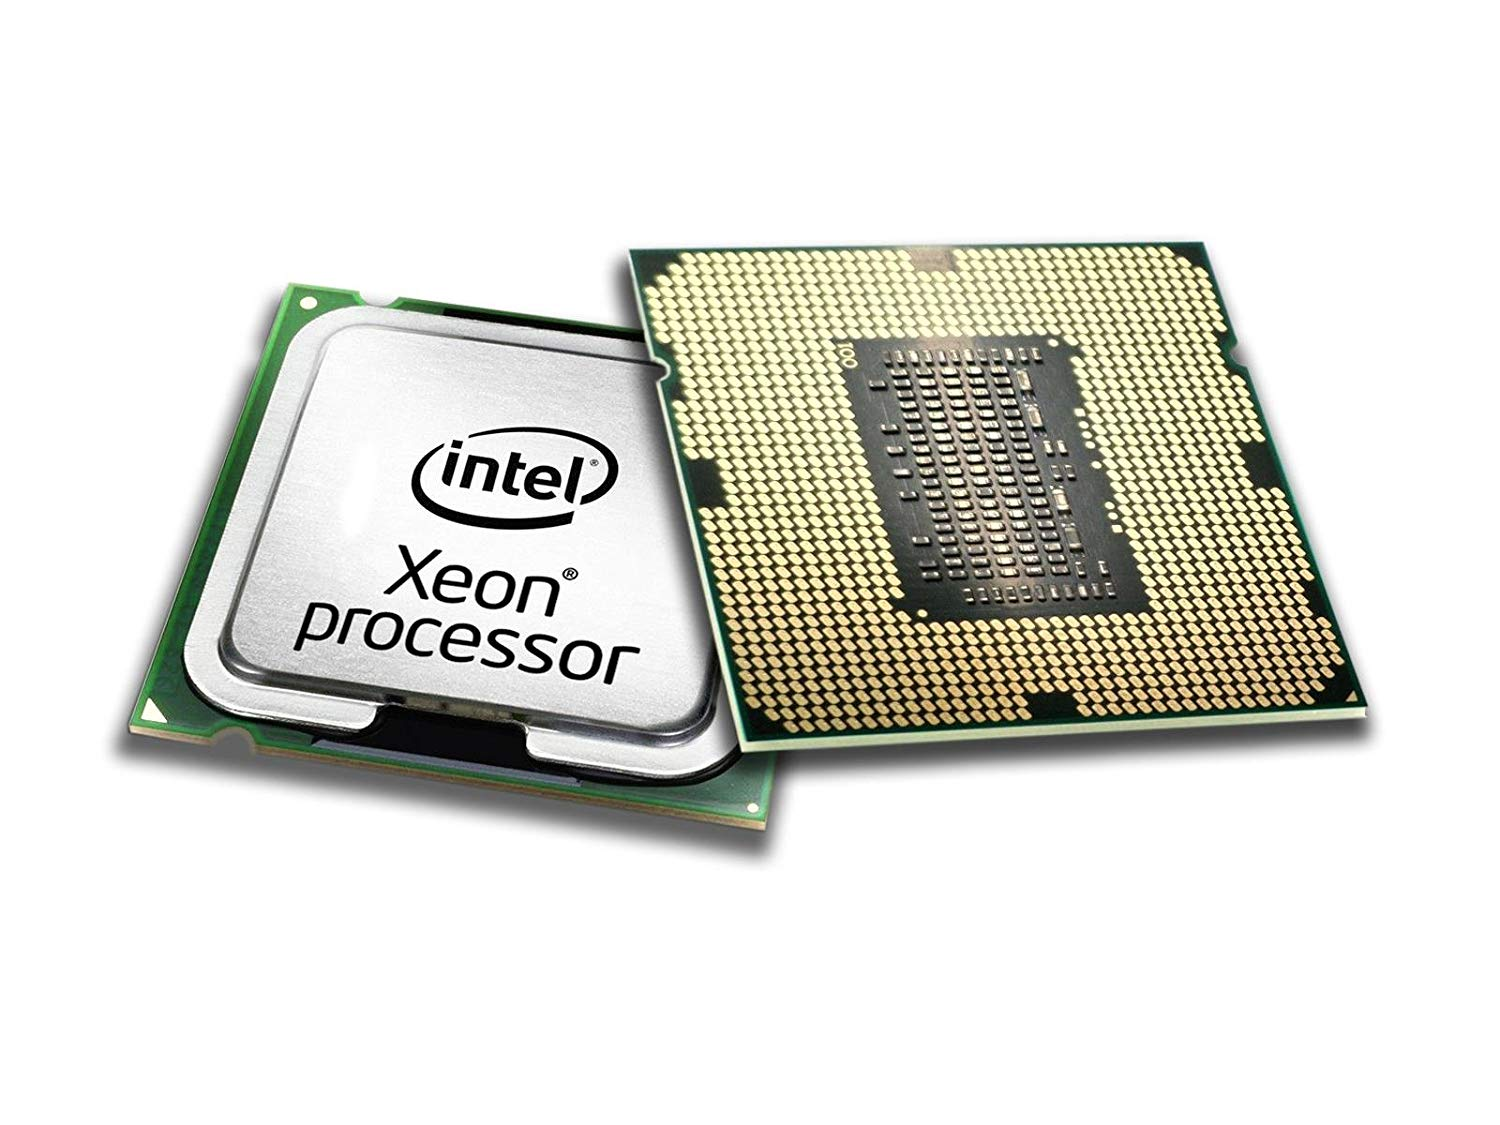
\includegraphics[height=1cm]{images/cpu.jpg}};
      }
      \uncover<3->{\draw[<->,thick] (memory) -- (cpu);}
      \uncover<4->{
        \node[tape,draw,thick,minimum height=1.5cm,minimum width=2cm,fill=green,right=of cpu.north east,yshift=-1cm] (input) {Input};
        \node[tape,draw,thick,minimum height=1.5cm,minimum width=2cm,fill=green,right=of cpu.south east,yshift=1cm] (output) {Output};
        \draw[<-,thick] (cpu) -- (input);
        \draw[->,thick] (cpu) -- (output);
        \node[above=of input,outer sep=0pt,inner sep=0pt] (keyboard) {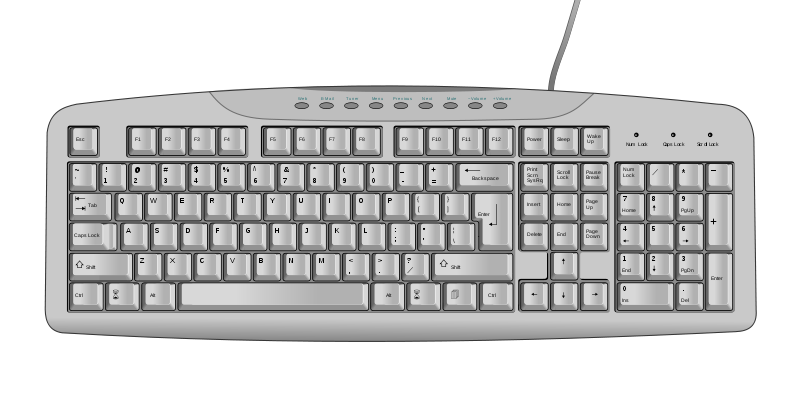
\includegraphics[height=1cm]{images/keyboard.png}};
        \node[right=0pt of keyboard] (mouse) {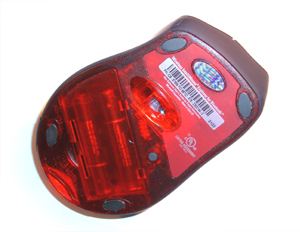
\includegraphics[height=1cm]{images/mouse.jpg}};
        \node[below right=0pt and 0pt of mouse,xshift=-.5cm] (monitor) {
\includegraphics[height=1cm]{images/monitor.png}};
        \node[below=0pt of monitor] (harddisk) {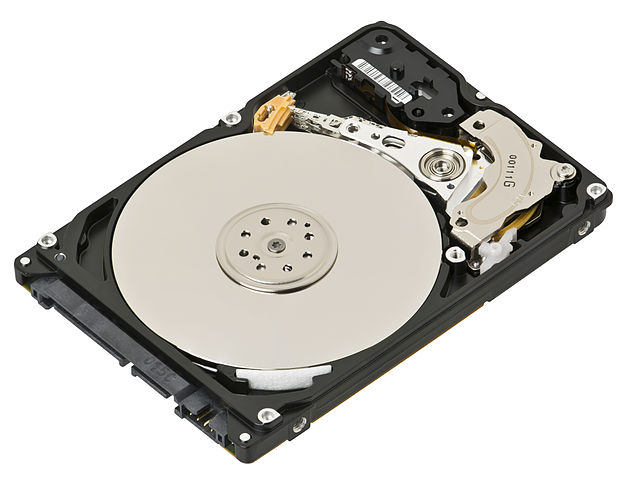
\includegraphics[height=1cm]{images/harddisk.jpg}};
        \node[below=0pt of harddisk] (usb-stick) {
\includegraphics[height=1cm]{images/usb-stick.png}};
        \node[below=0pt of usb-stick] (router) {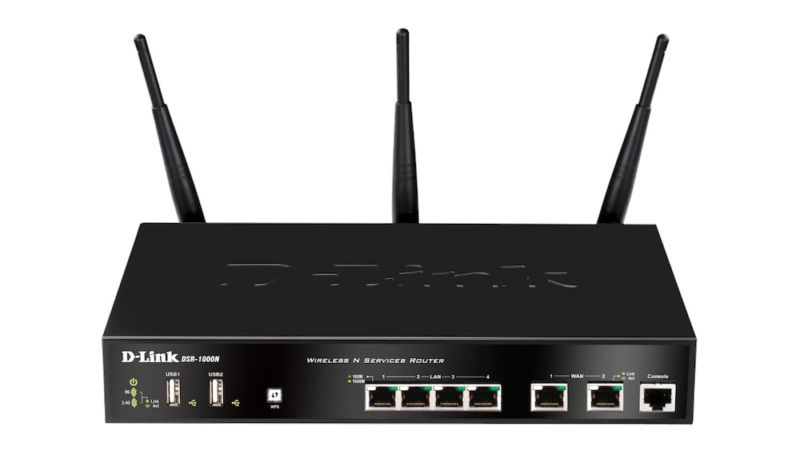
\includegraphics[height=1cm]{images/router.jpg}};
        \node[below left=0pt and 0pt of router] (gpu) {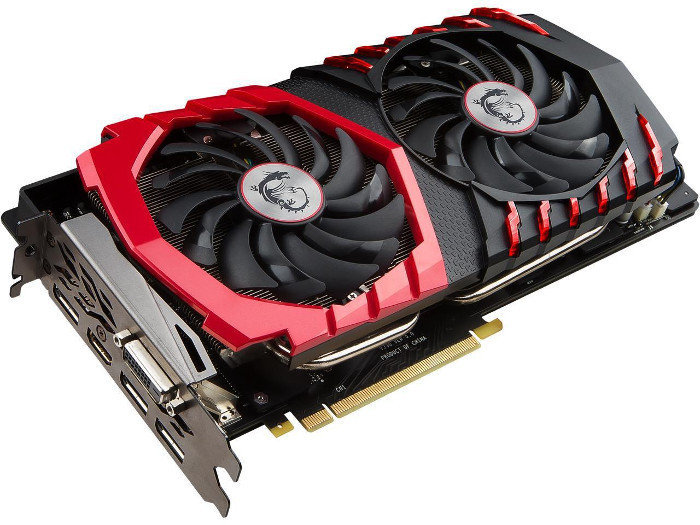
\includegraphics[height=1cm]{images/gpu.jpg}};
        \node[left=0pt of gpu] (sensor) {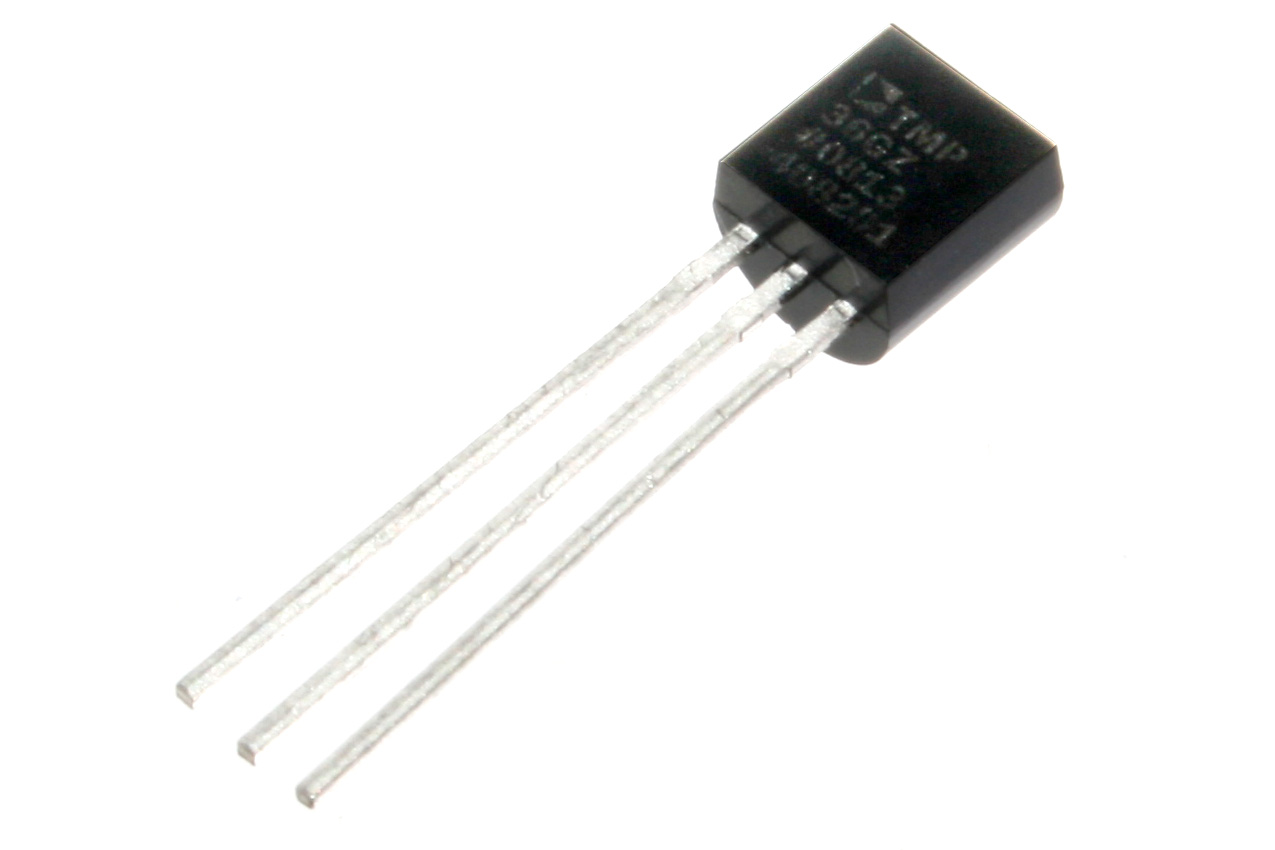
\includegraphics[height=1cm]{images/sensor.jpg}};
      }
    \end{tikzpicture}
  \end{center}

\end{frame}

\begin{frame}{The Von Neumann architecture \insertcontinuationtext}

  \begin{itemize}[<+->]
  \item Imagine memory as a looooong tape divided into locations whose content
    you can read and write
  \item Each memory location is identified by an index
    \begin{itemize}[<.->]
    \item e.g. location at position 8'363'944
    \end{itemize}
  \item Programs and the data they manage stay both in memory, typically in
    different regions
  \item The CPU fetches instructions from memory into its registers and executes
    them
  \item Typical instructions:
    \begin{itemize}[<.->]
    \item read data from memory into registers
    \item write data from registers to memory
    \item manipulate data in registers
    \end{itemize}
  \end{itemize}
\end{frame}

\begin{frame}[fragile]{Also data are binary}

  \begin{semiverbatim}
{\color{gray}00101001110110011000011111010111001011100111101100
11101000101001101011100111111100011101001000011010
00000110001101000011111010010001000101110000010010
00111011010111101101111110110011011111101100101101
10010010110011001101110011000011001011000001010010
11110100101111010001111001011000000000001111110100
1001110110001101101001\tikzref{ins}0110000101101111000000001101
00010001111001101000111100100110110110001101100100
01000110010111100011100010100101011011000110010001
10100011111101101000000000111101000001000100101101
00001001111011000000110000100110000101000100111011}\end{semiverbatim}

\uncover<2->{
  \tikz[overlay] \node[draw,thick,rounded corners,red,minimum width=65mm,minimum
  height=5mm] (data) at (ins) {};
}

\begin{itemize}
\item<3-> read as \alert<3>{integer number} the value is $1667850607$
\item<4-> read as \alert<4>{floating-point number} the value is $4.30511 \times 10^{21}$
\item<5-> read as \alert<5>{character string} the value is ``ciao''
\end{itemize}
\end{frame}

\begin{frame}[fragile]{A minimal C++ program}

  \begin{itemize}
  \item This program does nothing, successfully (details will be explained)
    \begin{codeblock}
int main() \{\}\end{codeblock}

  \item<2-> Let's write these 13 characters (including spaces) in a \alert{source
      file}, which we call \code{minimal.cpp}, using Visual Studio Code

    \begin{shellblock}<3->{
\$\tikzref{prompt}
\uncover<4->{\$ code minimal.cpp \inserthitenter\tikzref{command}}
\uncover<6->{\$ cat minimal.cpp \inserthitenter\tikzref{cat}
int main() \{\}
\$}}\end{shellblock}

\uncover<3>{\tikz[remember picture,overlay] \draw[<-,white] ([xshift=1ex] prompt) -- +(.5,0) node[white,right] {\scriptsize this is the shell prompt};}
\uncover<4>{\tikz[remember picture,overlay] \draw[<-,white] ([xshift=1ex] command) -- +(.5,0) node[white,right] {\scriptsize write this command (hit ``Enter'' at the end)};}
\uncover<6>{\tikz[remember picture,overlay] \draw[<-,white] ([xshift=1ex] cat) -- +(.5,0) node[white,right] {\scriptsize the cat command shows the contents of a text file};}

  \item<7> Before \alert{executing} the program we need to translate it into
    the language of the computer
  
  \end{itemize}

\end{frame}

\begin{frame}[fragile]{A minimal C++ program \insertcontinuationtext}

  \begin{itemize}

  \item In C++ the translation into a binary format is the job of the compiler,
    which produces an \alert{executable} file

\begin{center}
    \begin{tikzpicture}[every text node part/.style={align=center}]
      \node[tape,tape bend height=.3cm,draw,thick,inner sep=2pt,minimum height=2cm,minimum width=3cm] (source) {Source file \\ {\scriptsize(\code{minimal.cpp})}};
      \node[tape,tape bend height=.3cm,black,draw,thick, inner sep=2pt,minimum height=2cm,minimum width=3cm,right=3cm of source] (exe) {Executable binary file \\ {\scriptsize(\code{a.out})}};
      \draw[->] (source) -- (exe) node[above,align=center,midway] {Compilation \\ {\scriptsize(\code{g++})}};
    \end{tikzpicture}
  \end{center}

  \begin{shellblock}<2->{
\$ g++ minimal.cpp
\$ \uncover<3->{ls
a.out  minimal.cpp
\$ }\uncover<4->{./a.out\tikzref{program}
\$ }\uncover<5->{g++ minimal.cpp -o minimal
\$ ls
a.out  minimal  minimal.cpp
\$ }\uncover<6->{./minimal
\$ }}\end{shellblock}

  \uncover<4>{\tikz[remember picture,overlay] \draw[<-,white] ([xshift=1ex] program) -- +(1,0) node[white,right] {\scriptsize this command executes the program};}

  \item<7-> The \code{-o} option passed to the \code{g++} command allows to give
    another name to the final executable
  \end{itemize}

\end{frame}

\begin{frame}[fragile]{Spaces}

  \begin{itemize}
  \item Spaces are (almost) irrelevant
  \end{itemize}

  \begin{columns}[T]
  \begin{column}{.3\textwidth}<2->
    \begin{codeblock}
int main()\{\}

\end{codeblock}
  \end{column}

  \begin{column}{.3\textwidth}<3->
    \begin{codeblock}
int
main(  ) \{
   \}\end{codeblock}
  \end{column}

  \begin{column}{.3\textwidth}<4->
    \begin{codeblock}
int\tikzref{n1}main()\{ \}

    \end{codeblock}
  \end{column}

  \uncover<5->{
\begin{tikzpicture}[remember picture,overlay]
  \node[circle,radius=7pt,draw,red,line width=1pt,opacity=.7] at (n1) (n2){};
  \node[above=of n2,draw=red,line width=1pt,opacity=.7,rounded corners] {space needed here} edge[->,line width=1pt,red,opacity=.7] (n2);
\end{tikzpicture}
  }

\end{columns}

\begin{itemize}[<6->]
\item Tools exist to consistently format source code to improve readability
  \begin{itemize}
  \item They are customizable
  \item You are \textbf{required} to use them
  \end{itemize}
\end{itemize}

\begin{columns}[T]
  \begin{column}{.4\textwidth}
    \begin{shellblock}<7->{
\$ clang-format minimal.cpp
int main()
\{
\}
\$}\end{shellblock}
  \end{column}

  \begin{column}{.6\textwidth}
  \begin{codeblock}<8->{
# .clang-format file
\ldots
AllowShortFunctionsOnASingleLine: false
BraceWrapping:
  AfterFunction:   true
  \ldots}\end{codeblock}
  \end{column}
\end{columns}

\end{frame}

\begin{frame}[fragile]{Syntax check}

  \begin{itemize}
  \item The compiler can translate a program into a binary executable only if the
    code is syntactically correct

  \begin{codeblock}<2->{
intmain() \{\}}\end{codeblock}

  \begin{shellblock}<2->{
\$ g++ minimal.cpp
minimal.cpp:1:9: error: ISO C++ forbids declaration of \upquote{intmain} with \ldots
    1 | intmain() \{\}
      |         ^
\$}\end{shellblock}

  \item<3-> Error messages are usually precise about the cause of the error, but
    not always
  \item<3-> Learn to interpret error messages
  \end{itemize}

\end{frame}

\begin{frame}[fragile]{Comments}

  \begin{itemize}

  \item Code can contain comments

    \begin{codeblock}<2->{
int main() \alert{//} comment until the end of the line
\{
\}}\end{codeblock}

    \begin{codeblock}<3->{
int main()
\{
  \alert{/*} possibly multi-line comment
     that goes until the final marker
     and cannot nest \alert{*/}
\}}\end{codeblock}

  \item<4-> Comments are ignored by the compiler and are equivalent to spaces
  \item<4-> Comment are for humans
    \begin{itemize}
    \item Prefer expressive code
    \end{itemize}
  \end{itemize}

\end{frame}

\begin{frame}[fragile]{Basic notions of Input and Output}

  \begin{itemize}
  \item The input and output system allows a program to interact with the
    external world
  \item One mechanism offered by C++ to do input and output is the \textit{I/O
      streams} interface, which allows the creation and the manipulation of
    \textit{stream} entities
    \begin{itemize}
    \item Values are extracted from an input stream
    \item Values are inserted into an output stream
    \end{itemize}
  \item Input and output streams connected to the terminal are automatically
    available to a program
    \begin{itemize}
    \item \code{std::cin}, \code{std::cout} (and \code{std::cerr} for errors)
    \end{itemize}
  \item To extract and insert values, use the stream \textit{operators}
    \code{>>} and \code{<<}, respectively
  \end{itemize}

\end{frame}

\begin{frame}[fragile]{Hello}

  A less minimal C++ program (details will be explained)

  \begin{codeblock}
\alert<2>{#include <iostream>}\uncover<2->{ // import I/O utilities}
\alert<2>{#include <string>}\uncover<2->{ // import string utilities}

int \alert<3>{main}()\uncover<3->{ // start the program from here}
\{
\alert<4>{  std::cout <{}< "What\textquotesingle{}s your name? ";}\uncover<4->{ // print a message on the terminal}
\alert<5>{  std::string name;}\uncover<5->{ // some space is needed in memory for a string}
\alert<6>{  std::cin >{}> name;}\uncover<6->{ // read a string from the terminal into that space}
\alert<7>{  std::cout <{}< "Hello, " <{}< name <{}< \bslashn{};}\uncover<7->{ // print a multi-part message}
\}\end{codeblock}

\begin{shellblock}<8->{
\uncover<8->{\$ g++ hello.cpp -o hello \inserthitenter
\$ }\uncover<9->{./hello \inserthitenter
What\textquotesingle{}s your name? }\uncover<10->{Francesco \inserthitenter
Hello, Francesco
\$ }}\end{shellblock}

\end{frame}

\begin{frame}{Objects}

  \begin{itemize}[<+->]
  \item The constructs in a C++ program create, destroy, refer to, access,
    and manipulate \alert<.>{objects}
  \item An object is a region of storage (i.e. memory)
    \begin{itemize}[<+->]
    \item has a \alert<.>{storage duration}/\alert<.>{lifetime}
    \item has a \alert<.>{type}
    \item can have a \alert<.>{name}
    \end{itemize}
  \end{itemize}

\end{frame}

\begin{frame}{Types}

  \begin{itemize}[<+->]
  \item A type gives meaning to a piece of storage
    \begin{itemize}
    \item What's the meaning of a piece of storage that contains the sequence of
      bits $01100011011010010110000101101111$?
    \item Read as a sequence of alphabetic characters, it's the letters
      \textit{c}, \textit{i}, \textit{a}, \textit{o}
    \item Read as an integer number, it's $1667850607$
    \item Read as a floating-point number, it's about $4.30511 \times 10^{21}$
    \end{itemize}
  \item A type identifies a set of values and the operations that can be applied
    to those values
    \begin{itemize}
    \item C++ is a \alert{strongly typed} language (mostly)
    \end{itemize}
  \item The compiler checks that program instructions are compatible with the type system
    \begin{itemize}
    \item C++ is a \alert{statically typed} language (mostly)
    \end{itemize}
  \item A type is also associated with a machine representation for
    the values belonging to the type
  \item C++ defines a few fundamental types and provides mechanisms to build
    compound types on top of them
  \end{itemize}

\end{frame}

\begin{frame}{Fundamental types}
  \begin{itemize}
    \item arithmetic types
      \begin{itemize}
        \item integral types
          \begin{itemize}
          \item signed integer types: \code{short int}, \alert<3->{\code{int}},
            \code{long int}, \code{long long int}
          \item unsigned integer types: \code{unsigned short int},
            \code{unsigned int}, \code{unsigned long int}, \code{unsigned long
              long int}
          \item character types: \alert<3->{\code{char}}, \code{signed char},
            \code{unsigned char}, \ldots
          \item boolean types: \alert<3->{\code{bool}}
          \end{itemize}
        \item floating-point types: \code{float}, \alert<3->{\code{double}}, \code{long double}
      \end{itemize}
    \item \code{std::nullptr_t}
    \item \code{void}
  \end{itemize}

  \pause

  In general, size and machine representation are not defined by the
  standard

\end{frame}

\begin{frame}[fragile]{\code{int}}

  \begin{columns}
    \begin{column}{.8\textwidth}
      Type representing a signed integer number

      \begin{itemize}
      \item<2-> Set of values: subset of $\mathbb{Z}$
      \item<3-> Operations: addition, subtraction, multiplication, division,
        remainder, comparisons, \ldots
      \item<4-> Representation: 2's complement
      \item<5-> With N bits, values are in the range $[-2^{N-1}, 2^{N-1}-1]$
      \item<6-> Intended to have the natural size suggested by the architecture.
        Typical size is 32 bits (4 bytes)
        \begin{itemize}
        \item $[-2$ $147$ $483$ $648, +2$ $147$ $483$ $647]$
        \end{itemize}
      \end{itemize}
    \end{column}
    \hfill
    \begin{column}{.2\textwidth}
      \uncover<4->{\begin{tabular}{ r | r }
        7 & \alert{0}111 \\
        6 & \alert{0}110 \\
        5 & \alert{0}101 \\
        4 & \alert{0}100 \\
        3 & \alert{0}011 \\
        2 & \alert{0}010 \\
        1 & \alert{0}001 \\
        0 & \alert{0}000 \\
        -1 & \alert{1}111 \\
        -2 & \alert{1}110 \\
        -3 & \alert{1}101 \\
        -4 & \alert{1}100 \\
        -5 & \alert{1}011 \\
        -6 & \alert{1}010 \\
        -7 & \alert{1}001 \\
        -8 & \alert{1}000
      \end{tabular}}
    \end{column}
  \end{columns}

\end{frame}

\begin{frame}{Identifiers}

  \begin{itemize}
  \item An \textit{identifier} is a sequence of letters (including \code{_}) and
    digits, starting with a letter
    \begin{itemize}
    \item Avoid \code{_} at the beginning
    \end{itemize} 

  \item Identifiers are used to name entities in a program
    \begin{itemize}
    \item Choose meaningful names
    \end{itemize}
  \end{itemize}

\end{frame}

\begin{frame}[fragile]{Variables}

  \begin{itemize}
  \item A variable is an identifier that gives a \alert{name} to an
    \textit{object}
  \end{itemize}

  \begin{codeblock}<2->{
\uncover<2->{int i;            // declaration}\uncover<3->{; the value is undefined}
\uncover<4->{i = 4321;         // assignment of a constant}
\uncover<5->{int j\{1234\};   // declaration and initialization in one step}
\uncover<6->{i = j;            // assignment of j\textquotesingle{}s value to i}}\end{codeblock}

  \begin{tikzpicture}[
      mem/.style={
        node font=\ttfamily\scriptsize,
        minimum height=.5cm,
      },
      location/.style={
        mem,
        draw=black!50,
        minimum width=1.2cm,
        fill=green!20!white,
      },
      every node/.style={
        mem,
      },
      anchor=south west,
      node distance=0,
    ]
    \clip (0.1,-1) rectangle (\textwidth-0.1cm,1.5);
    %% \visible<3->{\draw[step=.5cm,gray,thin,dashed] (0, .1cm) grid (\textwidth,0.4cm);}
    \visible<2->{\node at (0,0) [mem,draw=black!50,minimum width=\textwidth,
        "Memory" above] {};}
      \visible<2->{\node at (2,0) [location, "i" below] {
          \alt<-2>{}{\alt<3>{?}{\alt<4-5>{4321}{1234}}}};}
        \visible<5->{\node at (7,0) [location, "j" below] {1234};}
  \end{tikzpicture}

  \uncover<7->{NB At the end \code{i} and \code{j} have the same value but remain
  \alert{distinct} objects}

\end{frame}

\begin{frame}{Keywords}

  The following identifiers are reserved
  \vskip .5cm

  {
    \setbeamerfont{localfont}{size=\scriptsize,family=\tt}
    \usebeamerfont{localfont}

    \begin{tabular}{l l l l l l}
      alignas  & const        & for       & private          & throw    \\
      alignof  & constexpr    & friend    & protected        & true     \\
      and      & const_cast   & goto      & public           & try      \\
      and_eq   & continue     & if        & register         & typedef  \\
      asm      & decltype     & inline    & reinterpret_cast & typeid   \\
      auto     & default      & int       & return           & typename \\
      bitand   & delete       & long      & short            & union    \\
      bitor    & do           & mutable   & signed           & unsigned \\
      bool     & double       & namespace & sizeof           & using    \\
      break    & dynamic_cast & new       & static           & virtual  \\
      case     & else         & noexcept  & static_assert    & void     \\
      catch    & enum         & not       & static_cast      & volatile \\
      char     & explicit     & not_eq    & struct           & xor      \\
      char16_t & export       & nullptr   & switch           & xor_eq   \\
      char32_t & extern       & operator  & template         & wchar_t  \\
      class    & false        & or        & this             & while    \\
      compl    & float        & or_eq     & thread_local
    \end{tabular}
  }
\end{frame}

\begin{frame}{Literals}

  A literal is a constant \textbf{value} of a certain \textbf{type} included in
  the source code

  \pause

  \begin{itemize}
  \item integer
  \item floating point
  \item character
  \item string
  \item boolean
  \item \code{nullptr}
  \end{itemize}

\end{frame}

\begin{frame}{Integer literals}

  \begin{description}[<+->]
  \item[decimal] non-\code{0} decimal digit followed by zero or more digits
    \begin{itemize}[<.->]
    \item \code{1 -98 123456789 -1\textquotesingle{}234\textquotesingle{}567\textquotesingle{}890}
    \end{itemize}
  \item[binary] \code{0b} or \code{0B} followed by binary digits
    \begin{itemize}[<.->]
    \item \code{0b1101111010101101 0B111\textquotesingle{}0101\textquotesingle{}1011\textquotesingle{}1100\textquotesingle{}1101\textquotesingle{}0001\textquotesingle{}0101}
    \end{itemize}
  \item[exadecimal] \code{0x} or \code{0X} followed by hexadecimal digits
    \begin{itemize}[<.->]
    \item \code{-0xdead 0xDEad123f 0XdeAD\textquotesingle{}123F}
    \end{itemize}
  \item[octal] \code{0} followed by octal digits
    \begin{itemize}[<.->]
    \item \code{01 -077 07\textquotesingle{}654\textquotesingle{}321}
    \item N.B. A \code{0} in front of a number is meaningful!
    \end{itemize}
  \end{description}

  \uncover<+->{Integer literals are of type \code{int}}

\end{frame}

\begin{frame}[fragile]{\code{std::string}}

  \begin{itemize}[<+->]

  \item A \textit{compound} (\textit{user-defined}) type to represent a
    string of characters
  \item Provided by the C++ Standard Library
  \item Many operations available
  \item An \code{std::string} can be initialized with a string literal, a
    sequence of escaped or non-escaped characters between double quotes
    \begin{itemize}[<.->]
    \item \code{"hello" "hello\bslashn{}world" "hello
        \bslash{"}world\bslash{"}"}
    \item \code{\bslash{}n} means ``newline''
    \end{itemize}
  \item The type of a string literal is \textbf{not} \code{std::string}
  \end{itemize}

  \begin{codeblock}<+->{
std::string corso = "Programmazione per la Fisica";
\uncover<+->{corso = corso \tikzref{strplusref}+ "\bslash{n}Anno Accademico 2022/2023";}}\end{codeblock}

\uncover<+->{
  \begin{tikzpicture}[remember picture,overlay]
    \node[draw=red,line width=1pt,opacity=.7,rounded corners, minimum
    width=1.5ex] at ([xshift=.5ex]strplusref) (strplusbox) {};
    \node[below=of strplusbox,draw=red,line width=1pt,opacity=.7,rounded
    corners] {concatenate} edge[->,line width=1pt,red,opacity=.7] (strplusbox)
    {};
  \end{tikzpicture}
}

\end{frame}

\begin{frame}[fragile]{Expressions}

  \begin{itemize}
  \item An expression is a sequence of operators and their operands
    that specifies a computation
  \item Literals and variables are typical operands, but there are others

  \begin{codeblock}<2->{
\uncover<2->{1 + 2}
\uncover<3->{\alert<8->{i = 1 + 2}       // assignment}
\uncover<4->{i == j          // equality comparison}
\uncover<5->{sqrt(x) > 1.42}
\uncover<6->{\alert<8->{std::cout <{}< "hello, " <{}< name <{}< \upquote{\bslash{}n}}}}\end{codeblock}

\item<7-> The evaluation of an expression typically produces a result
\item<8-> Some expressions have \textit{side-effects}
  \begin{itemize}
  \item They modify the state of the program, i.e. the state of memory, or the
    external world
  \end{itemize}

\end{itemize}

\end{frame}
